\documentclass[xetex,mathserif,serif]{beamer}
\usepackage{polyglossia}
\setdefaultlanguage[babelshorthands=true]{russian}
\usepackage{minted}

\useoutertheme{infolines}

\setmainfont{FreeSans}
\newfontfamily{\russianfonttt}{FreeSans}

\title{Хорошие практики тестирования и ООП}
\author[Юрий Литвинов]{Юрий Литвинов \newline \textcolor{gray}{\small\texttt{yurii.litvinov@gmail.com}}}
\date{03.04.2017г}

\begin{document}
	
	\frame{\titlepage}

	\section{Тестирование}

	\begin{frame}
		\frametitle{Тестирование, зачем}
		\begin{itemize}
			\item Любая программа содержит ошибки
			\item Если программа не содержит ошибок, их содержит алгоритм, который реализует эта программа
			\item Если ни программа, ни алгоритм ошибок не содержат, такая программа даром никому не нужна
		\end{itemize}
		Тестирование не позволяет доказать отсутствие ошибок, оно позволяет лишь найти ошибки, которые в программе присутствуют
	\end{frame}

	\begin{frame}
		\frametitle{Виды тестов}
		\begin{itemize}
			\item Модульные
			\item Интеграционные
			\item Системные
		\end{itemize}
		\begin{itemize}
			\item Регрессионные
			\item Приёмочные
			\item Дымовые (smoke-test)
		\end{itemize}
		\begin{itemize}
			\item UI-тесты
			\item Нагрузочные тесты
			\item ...
		\end{itemize}
	\end{frame}

	\begin{frame}
		\frametitle{Модульные тесты}
		\begin{itemize}
			\item Тест на каждый отдельный метод, функцию, иногда класс
			\item Пишутся программистами
			\item Запускаются часто (как минимум, после каждого коммита)
			\item Должны работать быстро
			\item Должны всегда проходить 
			\item Принято не продолжать разработку, если юнит-тест не проходит
			\item Помогают быстро искать ошибки (вы ещё помните, что исправляли), рефакторить код (``ремни безопасности''), продумывать архитектуру (мешанину невозможно оттестировать), документировать код (каждый тест --- это рабочий пример вызова)
		\end{itemize}
	\end{frame}

	\begin{frame}
		\frametitle{Почему модульные тесты полезны}
		\begin{itemize}
			\item Помогают искать ошибки
			\begin{itemize}
				\item Особо эффективны, если налажен процесс Continuous Integration
			\end{itemize}
			\item Облегчают изменение программы
			\begin{itemize}
				\item Помогают при рефакторинге
			\end{itemize}
			\item Тесты --- документация к коду
			\item Помогают улучшить архитектуру
			\item НЕ доказывают отсутствие ошибок в программе
		\end{itemize}
	\end{frame}

	\begin{frame}
		\frametitle{Best practices}
		\begin{itemize}
			\item Независимость тестов
			\begin{itemize}
				\item Желательно, чтобы поломка одного куска функциональности ломала один тест
			\end{itemize}
			\item Тесты должны работать быстро
			\begin{itemize}
				\item И запускаться после каждой сборки
				\begin{itemize}
					\item Continuous Integration!
				\end{itemize}
			\end{itemize}
			\item Тестов должно быть много
			\begin{itemize}
				\item Следить за Code coverage
			\end{itemize}
			\item Каждый тест должен проверять конкретный тестовый сценарий
			\begin{itemize}
				\item Никаких try-catch внутри теста
				\begin{itemize}
					\item \mintinline{java}|@Test(expected = NullPointerException.class)|
					\item Любая нормальная библиотека юнит-тестирования умеет ожидать исключения
				\end{itemize}
			\end{itemize}
			\item Test-driven development
		\end{itemize}
	\end{frame}

	\begin{frame}[fragile]
		\frametitle{Hamcrest}
		\begin{minted}{java}
assertThat(someString, is(not(equalTo(someOtherString))));
assertThat(list, everyItem(greaterThan(1)));
assertThat(cat.getKittens(), hasItem(someKitten));
assertThat("test", 
    anyOf(is("testing"), containsString("est")));
assertThat(x, 
    allOf(greaterThan(0), lessThanOrEqualTo(10)));
		\end{minted}
\end{frame}

	\begin{frame}
		\frametitle{Mock-объекты}
		\begin{itemize}
			\item Объекты-заглушки, симулирующие поведение реальных объектов и контролирующие обращения к своим методам
			\begin{itemize}
				\item Как правило, такие объекты создаются с помощью библиотек
			\end{itemize}
			\item Используются, когда реальные объекты использовать
			\begin{itemize}
				\item Слишком долго
				\item Слишком опасно
				\item Слишком трудно
				\item Для добавления детерминизма в тестовый сценарий
				\item Пока реального объекта ещё нет
				\item Для изоляции тестируемого объекта
			\end{itemize}
			\item Для mock-объекта требуется, чтобы был интерфейс, который он мог бы реализовать, и какой-то механизм внедрения объекта
		\end{itemize}
	\end{frame}

	\begin{frame}[fragile]
		\frametitle{Пример: Mockito}
		\begin{minted}{java}
@Test
public void test() throws Exception {
    // Arrange, prepare behaviour
    Helper aMock = mock(Helper.class);
    when(aMock.isCalled()).thenReturn(true);
    // Act
    testee.doSomething(aMock);
    // Assert - verify interactions (optional)
    verify(aMock).isCalled();
}
		\end{minted}
\end{frame}

	\begin{frame}
		\frametitle{Соотношение тестов}
		\begin{center}
			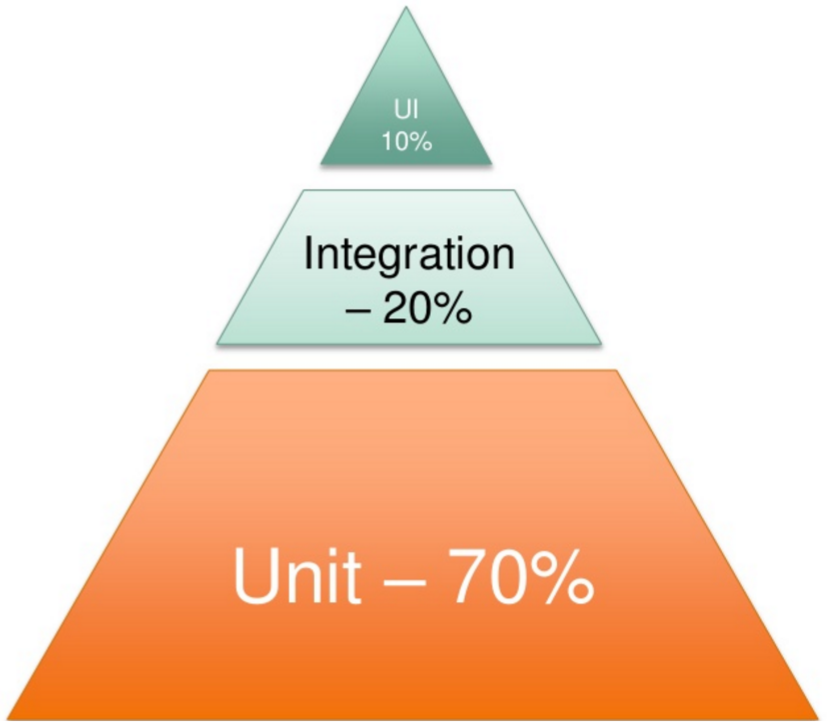
\includegraphics[width=0.6\textwidth]{testsProportions.png}
		\end{center}
	\end{frame}
	
	\section{Декомпозиция и модульность}

	\begin{frame}
		\frametitle{Модульность}
		\begin{itemize}
			\item Разделение системы на компоненты
			\item Потенциально позволяет создавать сколь угодно сложные системы
		\end{itemize}
		\vskip 1cm
		\begin{center}
			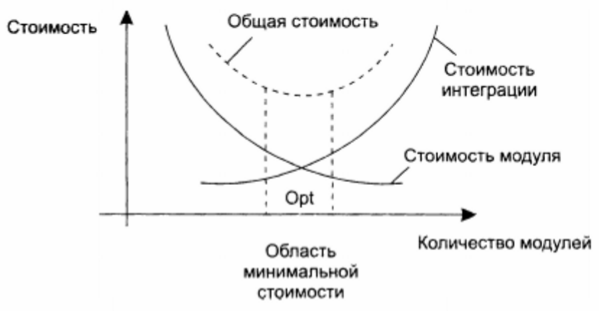
\includegraphics[width=0.5\textwidth]{modulesCost.png}
		\end{center}
	\end{frame}

	\begin{frame}
		\frametitle{Информационная закрытость}
		\begin{itemize}
			\item Со­держание модулей должно быть скрыто друг от друга
			\begin{itemize}
				\item Все модули независимы
				\item Обмениваются только информацией, необходимой для работы
				\item Доступ к операциям и структурам данных модуля ограничен
			\end{itemize}
			\item Обеспечивается возможность разработки модулей различными независимыми коллективами
			\item Обеспечивается лёгкая модификация системы
		\end{itemize}
	\end{frame}

	\begin{frame}
		\frametitle{Подходы к декомпозиции}
		\begin{itemize}
			\item Восходящее проектирование
			\item Нисходящее проектирование
			\begin{itemize}
				\item Постепенная реализация модулей
				\item Строгое задание интерфейсов
				\item Активное использование ``заглушек''
				\item Модули
				\begin{itemize}
					\item Четкая декомпозиция
					\item Минимизация
					\item Один модуль --- одна функциональность
					\item Отсутствие побочных эффектов
					\item Независимость от других модулей
					\item Принцип сокрытия данных
				\end{itemize}
			\end{itemize}
		\end{itemize}
	\end{frame}

	\begin{frame}
		\frametitle{Объекты}
		\begin{itemize}
			\item Objects may contain data, in the form of fields, often known as attributes; and code, in the form of procedures, often known as methods --- \textbf{\href{https://en.wikipedia.org/wiki/Object-oriented\_programming}{Wikipedia}}
			\item An object stores its state in fields and exposes its behavior through methods --- \textbf{\href{https://docs.oracle.com/javase/tutorial/java/concepts/object.html}{Oracle}}
			\item Each object looks quite a bit like a little computer --- it has a state, and it has operations that you can ask it to perform --- \textbf{\href{http://amzn.to/1PBmQpm}{Thinking in Java}}
			\item An object is some memory that holds a value of some type --- \textbf{\href{http://amzn.to/1XyGCtk}{The C++ Programming Language}}
			\item An object is the equivalent of the quanta from which the universe is constructed --- \textbf{\href{http://amzn.to/266oJr4}{Object Thinking}}
		\end{itemize}
	\end{frame}

	\section{Некоторые принципы ОО-проектирования}

	\begin{frame}
		\frametitle{Определение объектов реального мира}
		\begin{itemize}
			\item Определение объектов и их атрибутов
			\item Определение действий, которые могут быть выполнены над каждым объектом
			\item Определение связей между объектами
			\item Определение интерфейса каждого объекта
		\end{itemize}
		\begin{center}
			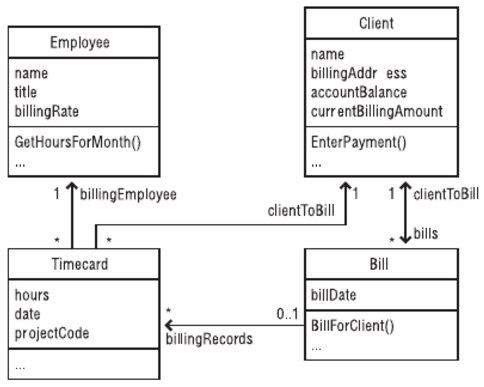
\includegraphics[width=0.4\textwidth]{billDomainModel.png}
		\end{center}
	\end{frame}

	\begin{frame}
		\frametitle{Согласованные абстракции}
		\begin{itemize}
			\item Выделение существенных характеристик объекта и игнорирование несущественных
			\item Определение его концептуальных границы с точки зрения наблюдателя
			\begin{itemize}
				\item Определение интерфейсов
			\end{itemize}
			\item Управление сложностью через фиксацию внешнего поведения
			\item Необходимы разные уровни абстракции
		\end{itemize}
		\begin{center}
			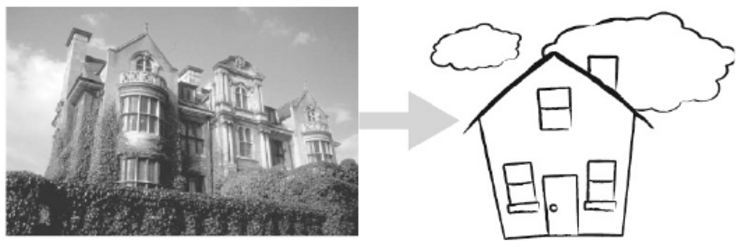
\includegraphics[width=0.55\textwidth]{abstraction.png}
		\end{center}
	\end{frame}

	\begin{frame}
		\frametitle{Инкапсуляция деталей реализации}
		\begin{itemize}
			\item Отделение друг от друга внутреннего устройства и внешнего поведения
			\item Изолирование контрактов интерфейса от реализации
			\item Управление сложностью через сокрытие деталей реализации
		\end{itemize}
		\vskip 1.5cm
		\begin{center}
			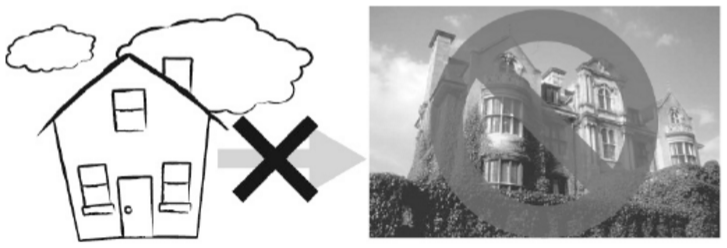
\includegraphics[width=0.55\textwidth]{incapsulation.png}
		\end{center}
	\end{frame}

	\begin{frame}
		\frametitle{Сокрытие ``лишней'' информации}
		\begin{columns}
			\begin{column}{0.65\textwidth}
				\begin{itemize}
					\item Изоляция ``личной'' информации
					\begin{itemize}
						\item секреты, которые скрывают сложность
						\item секреты, которые скрывают источники изменений
					\end{itemize}
					\item Барьеры, препятствующие сокрытию
					\begin{itemize}
						\item избыточное распространение информации
						\item поля класса как глобальные данные
						\item снижение производительности
					\end{itemize}
				\end{itemize}
			\end{column}
			\begin{column}{0.3\textwidth}
				\vskip 3cm
				\begin{flushright}
					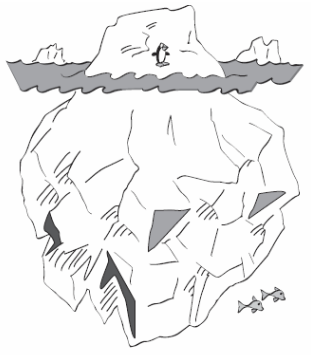
\includegraphics[width=\textwidth]{complexityHiding.png}
				\end{flushright}
			\end{column}
		\end{columns}
	\end{frame}

	\begin{frame}
		\frametitle{Изоляция возможных изменений}
		\begin{itemize}
			\item Определите элементы, изменение которых кажется вероятным
			\item Отделите элементы, изменение которых кажется вероятным
			\item Изолируйте элементы, изменение которых кажется вероятным
			\item Источники изменений
			\begin{itemize}
				\item Бизнес-правила
				\item Зависимости от оборудования
				\item Ввод-вывод
				\item Нестандартные возможности языка
				\item Сложные аспекты проектирования и конструирования
				\item Переменные статуса
				\item Размеры структур данных
				\item ...
			\end{itemize}
		\end{itemize}
	\end{frame}

	\begin{frame}
		\frametitle{Сопряжение и связность}
		\begin{itemize}
			\item \textbf{Сопряжение (Coupling)} --- мера того, насколько взаимозависимы разные модули в программе
			\item \textbf{Связность (Cohesion)} --- степень, в которой задачи, выполняемые одним модулем, связаны друг с другом
			\item Цель: слабое сопряжение и сильная связность
		\end{itemize}
	\end{frame}

	\begin{frame}
		\frametitle{Дополнительные принципы}
		\begin{itemize}
			\item Формализуйте контракты классов
			\item Проектируйте систему для тестирования
			\item Рисуйте диаграммы
		\end{itemize}
	\end{frame}

\end{document}